\documentclass[a4paper]{article}

\usepackage[eng,exjobb]{KTHEEtitlepage}
\usepackage[cp1252]{inputenc}
\usepackage[english]{babel}
\usepackage{fancyhdr}
\usepackage{graphicx}

\pagestyle{fancy}
\fancyhf{}
\rhead{}
\lhead{Sound validation of the clock-shift of the Manx Shearwater}
\rfoot{Page \thepage}

\begin{document}

                \ititle{Research Project}
              % \isubtitle{Julian Main, Lucas Van Berkel, Yorick De Boer, Amor Frans} % Optional
                \idate{Januari 2016}
                \irefnr{}
                \iauthor{\large{Sound validation of the clock-shift of the Manx Shearwater}}
                
                \makeititle

\newpage

%%%%%%%%%%%%%%%%%%
\tableofcontents
\newpage
%%%%%%%%%%%%%%%%%%
\begin{abstract}
    Bla bla blablabla bla bla bla blablablblabla bla blalblablalblalblalbablablalbblalblablbalablbalb blba bla bla b alblblbla bla bla bla bla blab alb alb alb alb alb albbla bla bla bla bla bla bla bla lb alb albblb alb blb alb bla blb alb 
\end{abstract}
%%%%%%%%%%%%%%%%%%
\addcontentsline{toc}{section}{Introduction}
\section*{Introduction}
The Manx Shearwater is a black and white seabird which nests in burrows. This bird nests on islands in the northeast Atlantic. In July, after the breeding period, the birds will migrate to the South-Atlantic and will return again in March the following year. During the breeding period one of the parents will stay with the eggs during a period of 7 to 12 days , while the other parent will search for food. After these 7-12 days the parents will swap roles.\\\\
Oliver Padget is a researcher at Oxford University and cooperates with IBED(Institute for Biodiversity and Ecosystem Dynamics) at Amsterdam. Padget wants to investigate whether this particular bird navigates using the sun. He is investigating this to attempt to gain more knowledge about this birds' way of navigating. Because the Manx shearwater breeds in burrows which are exposed to sunlight, the light can be easily manipulated by researchers, and therefore tests can be done to investigate the influence of sunlight on the birds their migration period.\\\\
One of the common nesting locations for the Manx shearwater is Skomer Island, which is a Welsh island. Skomer Island will be the location of the research. Here some of the burrows will be closed and artificial light will be placed in the burrows. To investigate the influence of the sun while the Manx shearwater navigate the time when the artificial light is on will be shifted in perspective to the time when the sun is up, this is called the clock-shift. The clock-shift is a good test because if the Manx shearwater uses the sun as a compass than the bird needs a precise endogenous clock to navigate. So if the researches successfully change the endogenous clock of the bird the influence should migrate differently. To prove this the birds were fitted with a GPS-tracker while the birds were migrating. The expectation of the researcher was that the route of the migration of the clock-shifted birds will differ from the normal birds. The result of this research showed that the clock-shifted birds indeed navigated differently comparing to the normal birds.\\\\
To give his results more validation Padget wanted to test if the clock-shift worked not only with GPS but also with sound recordings. The idea was that in each tested burrow a microphone would be inserted, and the microphone would record the sound in the burrow for 24 hours for several days. The recordings would be for the days where the time that the artificial light  is on matches the time when the sun is up, and also the shifted days would be recorded. Using machine learning algorithms it we attempted to evaluate whether the Manx shearwater has an activity pattern during the normal 24 hours and if that is the case  if it would be possible to conclude whether that pattern has shifted after the clock-shift. 



%%%%%%%%%%%%%%%%%%
\addcontentsline{toc}{section}{Problem}
\section*{Problem description}
As stated before, Oliver Padget wanted to validate whether the clock-shift has worked. Padget made recordings in 8 burrows. In each burrow the clockshift was manipulated. Two types of clock-shifts were used: a 4 hour forward shift(shift-fast), and a 4 hour shift backward shift(shift-slow). The recording in each burrow was a approximately 24 hours for 9 days. For the first six days the time when the light was on would match the time when the sun was up. In the last three days the clock would be shifted backwards or forward. The recordings were not complete for all burrows.\\\\
\begin{figure}[h]
\caption{Table of the data given by Oliver padget}
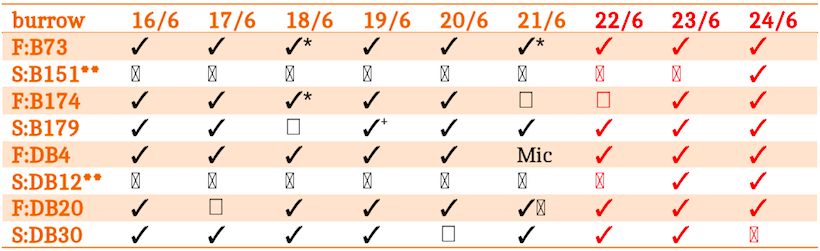
\includegraphics[scale=0.4]{table_of_birds.png}
\end{figure}

Padget's expectation was that the clock-shift would not work immediately, comparable with a jet-lag for human beings.
Padget also expected that the clock-shift would work, but in steps of 1 hour per day. This is a note that is important for the evaluation.\\\\
Padget wanted to investigate using the audio recordings whether there is a pattern in the activities of the bird and whether this pattern has shifted after the manipulation of the clock-shift. To determine the activity-pattern every activity in each recording was labeled. Each burrow had 24-hour recordings for 9 days, that means that there were approximately 216 hours of audio recording for all days. There were nine burrows so that is a total of 1944 hours of recordings. An audio analysis was done on the audio files, to classify the activity in the audio recordings. Four classes were used: bird shuffling, silence, environment noise, and bird calling. Machine learning was used to classify the recordings.\\\\
The main goal in this research was to validate whether the clock-shift worked or not based on the audio-recordings. To validate this the following sub-questions were attempted to answer:\\
 (I)    Is there a significant pattern of activity during 24-hours for the Manx Shearwater?\\
 (II)   If the answer in (I) is yes, will this pattern shift change after the clock-shift?\\


%%%%%%%%%%%%%%%%%%
\addcontentsline{toc}{section}{Method}
\section*{Method}
The research group got provided with the audio files of 8 different birds. Each microphone of each birds produced 9 audio files, each for every day the experiment contained. The first task was to think of the best way to find the pattern in the audio files. Previous work calculated the dominated frequency, the activity over a period of time using a amplitude threshold, the average amplitude over a period of time and the band power. Five minutes was the step time that was chosen to use, so that every interval provided enough information to calculate each feature. The result of the previous research concluded that the results were not reliable enough to define if the birds were clock-shifted or not. A different approach would be a better option. \\
Since the question of the research was to determine if the pattern of the birds was shifted, the research group decided to attempt the possibility to check if a certain noise was recorded in a audio file. If a certain noise is displayed more at certain times, a pattern is noticed and a shift can be determined. To attempt this method, a program online was used which uses 34 different short-period features, in order to determine if the sound tested, matches the sound classified. While listening to some audio files, multiple sounds could clearly be classified. The dominating sound was the noise or as classified for the program silence, when the bird moved it shuffles the microphone with created a very particular sound, the 'shuffle', also some microphones beeps and background noise were heard, both classified. Some of the features the program uses are the Zero Crossing Rate, Entropy of Energy and Spectral Spread. A complete overview of every feature is provided with the code. The step size this program uses was one second long, only to return a binary value of every second in the tested audio file. \\
A preliminary test of detecting 'shuffles' in a time frame of 241 seconds concluded that 90 percent of the 'shuffles' was detected in that time frame. Since the research group was provided the audio files in .mp3 format, and the chosen programming language python prefers .wav format, the audio files were converted. In order to maintain the time line of every bird and audio file, every recording was split into pieces of exact one hour long. Using the name of the files combining with the interval from the start of the original file, every audio file got its own unique start time. Every audio file, approximate $9\cdot8\cdot24=1728$ in total, was run through the program, delivering an array of 3600 entries long. Since two microphones of the eight did not work properly, the results of two birds had to be discarded Every entry then got labeled with its own unique time stamp and the array's were taped to together, to finally put the data in separate csv-files for every bird. The csv-files were later on put into a sql-database, in order to make it easier to retrieve data from certain time points.\\
From the sql-database every data point at a certain time at certain day from a specific bird could be accessed. The method chosen to analyse this data was to calculate the average of activity of every bird in its unshifted days separately, resulting in six different graphs. Since the resulting graphs showed a lot of variance from hour to hour, a moving average of five hours was calculated, showing a better perspective of the pattern of each bird. Plotting the pattern of the shifted days of the birds in the same graph, could show if the birds were clock-shifted.\\
http://www.ncbi.nlm.nih.gov/pmc/articles/PMC4676707/\\

\addcontentsline{toc}{subsection}{Environment}
\subsection*{Environment}

\addcontentsline{toc}{subsection}{Strategy}
\subsection*{Strategy}
%%%%%%%%%%%%%%%%%%
\addcontentsline{toc}{section}{Results}
\section*{Results}
%%%%%%%%%%%%%%%%%%
\addcontentsline{toc}{section}{Discussion}
\section*{Discussion}
%%%%%%%%%%%%%%%%%%
\addcontentsline{toc}{section}{Log}
\section*{Log}
\addcontentsline{toc}{subsection}{Week 1}
\subsection*{Week 1}
During the first meeting  the Oliver Padget and Emiel van Loon described the problem to us. Contact details and further appointments were made. We concluded that we would meet about two times each week and more if necessary. Oliver Padget is the main client and Emiel Van Loon is also involved in this project just in case Oliver Padget is not available or leaving the Netherlands.  We promised to send emails regularly with updates of our progress to the people involved in the project. For communication between group members we made a Whats-App group group chat, and also created a Github repository where the code and other files of our project would be stored. The plans we made, and tasks we assigned to each group member are in appendix I.\\\\
Last year a group of students also tried to solve the same problem, the report of this group has been sent to us. According to their results they have not been able to succesfully determine whether there was a clockshift. So we decided to try a different approach than them.
\\\\
The group of last year separated the data in smaller segments so the size of the files would be manageable. After the separation they classified each file and predicted whether the bird at that time perceived the moment as day or night. They used 3 features(amplitude, frequency and activity).\\\\
Before we determined our strategy we investigated which environment has the most potential to solve this problem. We chose to program in Python because we found an extensive library to analyze audio files (pyAudioAnalysis). The machine learning module in this library uses 64 features to analyze an audio file/segment. This is a big improvement to the 3 features of last year.\\\\
The pyAudioAnalysis only accepted .wav files as input, and not the .mp3 we were given. So we had to convert these files to .wav.\\\\
Before we started programming and analyzing the audio files we first determined a strategy. We had 3 options in mind:\\\\
1. The same strategy as last year: separate 24-hour fragments into smaller segments and classify them into day or night activity\\
\emph{In the report of last year we read that they faced many problems and the result were not as good as they hoped, so we decided to not try this option again although our data is better regarding to our client.}\\\\
2. Activity detector: Implement a threshold that is depending on features. If the audio file exceeds this threshold then this segment/point will be returned on the time-lines. then compare the time-lines of the normal clock and the shifted clock. If the shifted-clock time line differ from the normal then there is a signal that the clock-shift worked.\\\\
3. Supervised isolating distinctive sounds: Collect training data of distinctive sounds such as shuffling, calling and environment noise. Then let the program learn to recognize these sounds and make a vector over 24 hours of this classification. Then compare the vectors between normal vectors and the clock-shifted vectors. \\\\
We considered options 2 and 3 as the best strategy. But decided to choose for option 3, since this would be a more precise way than option 2. \\\\
When the strategy was chosen we started to collect the training data. We searched for distinctive sounds such as shuffling, calling, environment and silence. These fragments were mostly between 3 and  6 seconds long. We tested on two audio files:\\
- b73 the audio file of the first day, where there is no clock-shift. \\
- b73 the audio file of the last day, where the clock is shifted\\\\
We did this because in this way we also could test the compare method after the classification, so we could see if there were signs of the clock shift having worked or not. Because of the large files it is not possible to analyze more audio files before we were sure that the code worked well.\\\\
We started by converting the .mp3 to .wav. When that was done we started pyAudioAnalyis the algorithm to see if it could successfully shuffling. We used the pyAudioAnalysis library with the k-nearest neighbor algorithm. pyAudioAnalysis uses the values of 64 features at each point and classifies that as shuffling or silence. We started to classify only these two to see if our strategy has potential.  Our first test was to let the program recognize the sound of shuffling. We started with an accuracy of 33\% but after some fine tuning we reached an accuracy of 88\%.\\\\
After some testing and collecting training data we discovered that the .mp3 files contained errors. We decided to cut the audio .mp3 ausio files in segments of 1 hour and then convert these smaller files to .wav.\\\\
Another problem we were facing is that the program returns many false positives. A lot of fragments of class silence were classified as shuffling. Although the accuracy was 88\%, the accuracy might decrease alot if we increased the test set. Emile Van Loon also advised to look for a better algorithm than k-nearest neighbor. So we investigated which other algorithms can fit our program and our problem.\\\\
In our meetings this week with Oliver Padget we described our progress and our strategy. Padget approved our strategy and understood why we chose this strategy. He also recommended to analyze the difference between the day and night patterns between the normal and the clock-shifted audio files. We can do that using the information of the latitude and longitude of the location of the birds, the date/time the audio recorded started and information when on that particular day at that location sunset and sunrise took place.\\\\
In week 2 we planned to optimize our program trying other learning algorithms and run the program on a larger scale. We also want to choose a good strategy to compare the results. A possibility is using machine learning but because there are not many audio files it may be possible do it manually and visually. But that depends on the difference between the results of the normal files and the clock-shifted files. 

\addcontentsline{toc}{subsection}{Week 2}
\subsection*{Week 2}

Our main goal of week 2 is to get results on a single test bird/burrow b73. The group of last year collected all burrows and used all the data from separated burrows in one set.  The results of this strategy were not conclusive, but they also tested it on one particular burrow/bird. The results of the test on one burrow were better. So we decided to get training data from all burrows and test it both separately and combined. We also expect that the separated dataset will work better because each burrow can differ regarding to the size, the position of the microphone and other dependencies and therefore the recording of the sounds can be different.\\\\
After trying several tests running on only one hour of the recording we decided to run the program on the 24 hours recording for all days of burrow b73. The results were implement in a .csv data file so that we can plot the results using this data. The code has been made and implemented in this week. \\\\
Before the last meeting of week 2 with Oliver Padget we want to showed him the results the of burrow b73. We finished the code for the complete run on b73 and also implemented the code to plot and read the data from the .csv file. The following graph has been showed  to Oliver Padget at the last meeting of week 2:\\\\
* put first graph here\\\\
We added also the plot of the last day because the clock shift will not immediately work after 1 day. The expectation of the researcher is that the biological clock will shift 1 hour a day. \\\\
Oliver Padget was satisfied with the results and he saw signs that the clock shift has worked. Because b73 has been clock-shifted forward he expected to see the activity pattern shift to the left. He said that you can see the first peak shift to the left and therefore the results are hopeful. He advised us to normalize the data and also use average smoothing to get cleaner results and to see a better pattern/shift.\\\\
After the week 2 Oliver Padget returned to the UK and we agreed to communicate further on email and also continue our weekly meetings on Skype.\\\\
Regarding to the test results we discovered some errors. Some of the recording were not recording the full 24 hours, therefore some time segments returned no data. After implement code to fix this to program was ready to run on all burrows.\\\\
For each burrow the run-time is 5 hours, so we planned to run the computer the whole weekend and have the results in the beginning of week 3.\\\\
In week 3 we hope to have the complete results and conclude whether the clock-shift has worked or not. 

\addcontentsline{toc}{subsection}{Week 3}
\subsection*{Week 3}
\end{document}
